\section{Literature review} \label{sec:litrev}

In a preparation to choosing the right approach for this problem, a research on
the recent works and advances in autonomous drone racing has been conducted. A
selective literature review on the topic is given in details on
table~\ref{table:drone-racing-literature}. To select the most relevant papers related
to this thesis, whose focus is mainly on the perception and deep learning, most
papers that treated advanced control solutions were discarded. Using search
engines and keywords such as ``drone racing'', ``deep learning'', ``IROS'' and
the like, a dozen of results were found to begin the review. By looking into
the references of the most interesting papers, and mainly visiting the websites
of the research groups and authors, more interesting articles were found.

The result of this literature review is a deeper knowledge of how autonomous
drone racing is approached, and mainly what types of sensors are used to solve
this challenge efficiently. Surprisingly, only a few articles are accompanied
with the source code of the solution presented, which greatly narrows the
options to tackle the problem. The following section sums up the general
approach chosen by these papers.

%\newpage
\newgeometry{hmargin=2cm,vmargin=0.5cm}
\thispagestyle{lscape}

\begin{landscape}
	\centering
	\begin{longtable}{@{} p{7cm} p{4cm} p{1cm} p{10cm} p{5cm} @{}}
		\caption[Literature review]{Relevant autonomous drone racing articles: chronologically
		sorted} \label{table:drone-racing-literature}\\
		\hline
		\toprule
		Article	& University & Year & Description & Dataset\\ 
		\midrule
		Deep Drone Racing: Learning Agile Flight in Dynamic Environments
		& University of Zürich and ETH Zürich \& Intel Labs
		& June 2018 
		& The method makes use of a CNN to predict a goal direction in the
		local image coordinates, by taking a $300 \times 200$ RGB image as
		input, and outputting a tuple. The latter holds a direction vector, and
		a normalized desired speed vector. Then, a control system generates
		low-level commands from the given tuple. The desired speed is computed
		by scaling the predicted speed by a specified max speed.
		& Images collected from a real flight, and whose ground-truth was
		enhanced with an expert policy projection. It is a semi-synthetic
		dataset of real images and compute ground-truth. \\ 
		\addlinespace
		Beauty and the Beast: Optimal Methods Meet Learning for Drone Racing
		& University of Zürich and ETH Zürich \& Intel Labs
		& Oct. 2018
		& The method uses a combination of a deep neural network (CNN +
		$2\times$ MLP) regressing the mean and variance of a multivariate
		normal distribution describing the estimate of the next gate's pose,
		and an Extended Kalman Filter that estimates the joint probability
		distribution of a gate's pose. The perception system is never trained
		on data from tracks and environments it is later deployed in.  & Custom
		dataset from footage in 5 different environments (45,000 images from
		the front-facing camera) + on-board state estimation.\\
		\addlinespace
		Perception, Guidance, and Navigation for Indoor Autonomous Drone Racing Using
		Deep Learning
		& Unmanned Systems Research Group
		& July 2018
		& The method shows the great advantages of Single Shot Detector CNNs
		over the old-fashion color detection algorithms. It is able to pick the
		closest gate among overlapping gates, as well as cope with moving
		gates, and can therefore be applied to various environments: being
		static or dynamic. It also makes use of a Line-Of-Sight algorithm for
		guidance and control of the quadcopter.
		& Custom dataset of gates from footage filmed in various environments:
		1544 images were used to train the CNN for 12,000 iterations. For the
		testing, various background images, precisely 7380 frames, were used.\\
		\addlinespace
		Autonomous UAV Navigation Using Reinforcement Learning
		& \emph{Not specified}
		& Jan. 2018
		& The method demonstrates the use of Deep Reinforcement Learning for
		UAV navigation in unknown environments. It uses Q-Learning for
		computing the shortest path to a previously set target point, and a PID
		controller to smoothly hover over a 3D coordinate at each step of the
		algorithm. It is a simple application of Deep RL in which a drone goes
		from A to B using the shortest path, but it is not complex enough to
		navigate through obstacles or dynamic environments.
		& \emph{None needed.}\\
		\addlinespace
		Fast Efficient Object Detection Using Selective Attention
		& RMIT University, The University of Tokyo, IBM Research, UBTECH Sydney
		AI Center
		& Nov. 2018
		& The methods exposes the common bottleneck in state-of-the-art object
		detectors, and proposes a novel solution (based on recent study on the
		superior colliculus and the efficiency in human and primate visual
		systems) that is able to achieve saliency detection at the insane speed
		of 500 frames per second, making it very suitable for embedded systems.
		& COCO dataset\\
		\addlinespace
		Aggressive Deep Driving: Combining Convolutional Neural Networks and
		Model Predictive Control
		& Georgia Inst. Of Technology
		& July 2017
		& The method presents a deep learning based approach in aggressive
		driving for a rally car. It uses a CNN to generate a top-view, and a
		perspective view, of a cost function map that is used as input for the
		Model Predictive Path Integral Controller which generates the right
		trajectory for the car.
		& Custom dataset of 300,000 images with the corresponding pre-computed
		ground-truth cost maps.\\
		\addlinespace
		Deep Neural Network for Real-Time Autonomous Indoor Navigation
		& Cornell University
		& Nov. 2015
		& The method successfully learns from human pilots to drive a quadcoptor
		in a closed indoor environment, towards a target object, by using a
		common CNN architecture (ConvNet) to infer driving commands from an
		input RGB image.
		& Custom dataset of images from 7 indoor locations (corridor & corners)
		labeled with flight commands.\\
		\addlinespace
		Vision-Based Autonomous Mapping and Exploration Using a Quadrotor MAV
		& Computer Vision and Geometry Lab, ETH Zürich
		& Oct. 2012
		& The method shows how a front-looking stereo camera coupled with a
		downward-looking monocular camera can be used to offer autonomous
		mapping and exploration (on-board) via the Vector Field Histogram+ and
		Frontier-Based algorithms. They also compare those on-board algorithms
		with a Visual SLAM process running off-board, and provide satisfying
		results.
		& Custom dataset of more than 5000 stereo image pairs for the visual
		SLAM algorithm.\\
		\addlinespace
		DroNet: Learning to Fly by Driving
		& ETH Zürich
		& Jan. 2018
		& The method shows impressive results for a supervised learning
		algorithm (ResNet CNN) that learns from human drivers (cars and
		bicycles) to drive in  unstructured (city-like) environments, and can
		even perform well in previously unseen scenes. The CNN outputs velocity
		commands, which go through a low-pass filter, and a binary
		classification for the collision detection. The conclusion is that
		RL-based methods, when trained in simulation, suffer from the domain
		shift and might require real-world data to generalize, while supervised
		learning is a better way to learn effective flying policies.
		& 70,000 images of car driving from Udacity + custom footage of 32,000
		images from a GoPro on a bicycle for the collision dataset.\\
		\addlinespace
		GapFlyt: Active Vision Based Minimalist Structure-Less Gap Detection
		For Quadrotor Flight
		& \emph{Not specified}
		& Feb. 2018
		& The method addresses the problem of gap detection of an unknown shape
		and location with a monocular camera and on-board sensing. It uses a
		Temporally Stacked Spatial Parallax algorithm for detecting the gate
		(using a deep-learning based Optical Flow algorithm), and a visual
		servoing algorithm that is mostly convex optimization with a Kalman
		filter.
		& \emph{None needed.}\\
		\addlinespace
		Autonomous drone race:  A computationally efficient vision-based
		navigation and control strategy
		& TODO
		& TODO
		& TODO
		& TODO
		%\footnotetext{Continued on next page \ldots}
	\end{longtable}
\end{landscape}

\clearpage
\restoregeometry


\subsection{General approach}
As it can be seen from the preceding literature review, most robotic systems'
operation can be modeled by the commonly known \emph{sense, plan, act}
paradigm:

\begin{figure}[h]
	\centering
	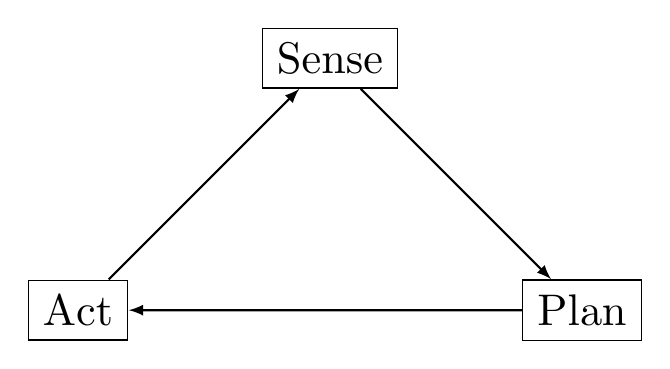
\begin{tikzpicture}[node distance=2cm,-latex, scale=1.6, every
		node/.style={scale=1.6}, box/.style = {draw,rectangle, minimum
		width=2cm}]
		\node[draw,rectangle] (sense) {Sense};
		\node[draw,rectangle,below of=sense,xshift=2cm] (plan) {Plan};
		\node[draw,rectangle,below of=sense,xshift=-2cm] (act) {Act};

		\draw[thick] (sense) -- (plan);
		\draw[thick] (plan) --(act);
		\draw[thick] (act) -- (sense);
	\end{tikzpicture}
	\caption{The sense, plan, act robotic paradigm.}
	\label{fig:robotic_paradigm}
\end{figure}

\begin{itemize}
	\item{\textbf{Sense}}: gather information using sensors (camera, IMU, sonar...).
	\item{\textbf{Plan}}: create a world model using all the information, and plan
		the next move.
	\item{\textbf{Act}}: carry out the actions that the plan calls for.
\end{itemize}

~\\
This thesis will be focused mainly on the sensing of the drone control, and
more precisely using deep learning and computer graphics. However, an important
part of the trajectory planning directly follows the sensing phase, therefore
those two first phases of the control loop can be included in the scope of the
project.

To this day, most drones in the robotic research field are running \emph{Robot
Operating System} (ROS),  which is a set of ``libraries and tools to help
software developers create robot applications''~\cite{ROS}. It allows to
independently run programs as ``nodes'', which can communicate with each other
using a principle of ``subscription'' and ``publication`` on easily definable
topics.

ROS makes the transition between the simulated environment and the real world
seamless, because it can be installed on most Linux systems, and adds a layer
of abstraction between the hardware and the software, by distributing packages
built by the community.\\

The implementation of the computer vision algorithms will be constrained within
ROS, and cooperate with the different control components, in an effective
modular manner.\\

As deep learning has known an exponential growth during the past decade,
computer vision applications tend to exploit the power of convolutional neural
networks more and more. Thanks to their impressive performance in specific
problem solving, CNNs are becoming the main choice for tasks such as object
detection, object segmentation, object recognition or object tracking.

In drone racing, the latest works, which are often the best performing, tend to
employ CNNs for the sensing part, or even as an all-in-one solution. It is a
reasonable choice mainly because neural networks are observed to offer
robustness and accuracy, to the cost of computational power. They can be hard
to train, given their sporadic nature, but it is often a very good alternative
to developing a custom algorithm which can take a lot of time and does not
guarantee consistent results, in different lighting conditions for instance.

On that note, the chosen method for solving the drone racing challenge is
using a convolutional neural network, coupled with a simple state-machine 
using a PID controller to steer the drone.
